\documentclass[11pt, letterpaper, twoside, openright]{book}

\usepackage{amscd}
\usepackage{amsfonts}
\usepackage{amsmath}
\usepackage{amsrefs}
\usepackage{amssymb}
\usepackage{amsthm}
\usepackage{array}
\usepackage{arydshln}
\usepackage{bbm}
\usepackage{calc}
\usepackage[labelformat=empty, font=bf]{caption}
\usepackage{color}
\usepackage{enumerate}
\usepackage{epsfig}
\usepackage{epstopdf}
\usepackage{etoolbox}
\usepackage{eucal}
\usepackage{fix-cm}
\usepackage{graphicx}
\usepackage{hyperref}
\usepackage{latexsym}
\usepackage{lscape}
\usepackage{mathrsfs}
\usepackage{multicol}
\usepackage{multirow}
\usepackage{pgfplots}
\usepackage{rotating}
\usepackage{setspace}
\usepackage{soul}
\usepackage{stmaryrd}
\usepackage{textcomp}
\usepackage{tikz}
\usepackage{verbatim}
\usepackage{vwcol}
\usepackage[all]{xy}
\usepackage{xparse}

\NewDocumentCommand{\projectchapter}{o m m}{%
\IfNoValueTF{#1}
{\chapter[#2]{#2\origtitle{#3}}}
{\chapter[#1]{#2\origtitle{#3}}}%
}
\newcommand\origtitle[1]{\\
\parbox{\textwidth}{\normalsize\vspace*{2\baselineskip}#1}}
%%%%%%% YOU SHOULDN'T NEED TO ADD ANY PACKAGES. IF YOU DO, PLEASE LET ME KNOW.




\let\TAB\tabular
\renewcommand\tabular{\noindent\TAB}    
\let\oldenumerate\enumerate
\renewcommand{\enumerate}{
  \oldenumerate
  \setlength{\itemsep}{1pt}
  \setlength{\parskip}{0pt}
  \setlength{\parsep}{0pt}
}
\pagestyle{myheadings} % I removed the header of the pages that showed the chapter title, but it also deleted the page subsections. Do we want this? - Mehul

\usetikzlibrary{chains,fit,shapes}
\usepackage{ulem}
\tikzstyle{tmtape}=[draw,minimum size=0.7cm]
\tikzstyle{large}=[minimum width=1.5cm]
\tikzstyle{current}=[draw=red!50]






\begin{document}
\mainmatter

\projectchapter{A Game We Can't Win: Undecidability of Quantificational Logic}
{Jonas Wechsler, Mehul Bhatnagar, Sam Grayson}

\begin{flushright}
\textit{"I know that I know nothing."} \\
- Socrates
\end{flushright}

General Todos: italicize the first instance of vocabulary words, format graphics better, refer to graphics as fig n, format theorems and defns, spellcheck.

\section{Computers}  %%USE SECTIONS AND SUBSECTIONS TO STRUCTURE YOUR PAPER
\subsection{Alan Turing's life}
%Is this too similar to wikipedia?
%\subsubsection{Early Life}

Alan Turing (born June 23, 1912 in London) demonstrated intelligence at an early age first at St. Micheal's then at Sherborne School. After grade school, Turing studied and subsequently taught mathematics at Cambridge University. At Cambridge, he wrote ``On Computable Numbers, with an Application to the Entscheidungsproblem'', a paper on the limits of proof and computation that created formal and simple hypothetical devices that ultimately became known as Turing Machines.

%Alan Turing was born on June 23, 1912 in London, while his father was on leave for his position in the Indian Civil Service. His father's civil service was active throughout Turing's childhood, so he and his brother stayed with a retired Army couple whle their parents were traveling. While growing up he attended a day school, St. Michael's, at the age of 6, where his skills in mathematics were well respected by the teachers. At the age of 13, he moved to Sherborne School, a well known independant boys public school. Unfortunately, science and math were not as respected at this school. Once, his headmaster wrote to his parents, "I hope he will not fall between two stools. If he is to stay at public school, he must aim at becoming educated. If he is to be solely a Scientific Specialist, he is wasting his time at a publicschool".

%\subsubsection{Life during World War II}

During World War II, he worked for the British to crack German codes at Bletchley Park. There he developed an early computer that could guess the key to decrypt the Enigma machine, providing the Allies with crucial information. He made these computers practical and had other contributions to cryptography for the  British. He was known by his coworkers for his quirky habits.

%In 1936, Turing moved to Princeton, though he returned to England in 1938, when he began working for the British cryptanalytic department in a secret part-time job for the Government Code and Cypher School. Following the onset of World War II, he began working full-time at the department's headquarters, Bletchley Park.

%At Bletchley he lead a team that developed a machine known as the bombe, to be used to decode German messages encoded by the Enigma machine. His machine worked and he managed to provide the Allies with crucial information. After his production of the bombe, he also deduced the indicator prodecedure made by the German navi, developed a statistical prodecure for efficient ue of the bombes, developed a prodecure for deducing cam settings of another German cypher (the Lorenz SZ 40/42), and developed a portable secure voice scrambler.
%I should reword that paragraph

%At Bletchley Turing was considered fairly eccentric. Jack Good, a coworker and fellow cryptanalyist, said about Turing that:

%\setlength{\leftskip}{1cm}
%``In the first week of June each year he would get a bad attack of hay fever, and he would cycle to the office wearing a service gas mask to keep the pollen off. His bicycle had a fault: the chain would come off at regular intervals. Instead of having it mended he would count the number of times the pedals went round and would get off the bicycle in time to adjust the chain by hand. Another of his eccentricities is that he chained his mug to the radiator pipes to prevent it being stolen.``
%\setlength{\leftskip}{0pt}

His work did not go unnoticed. In 1945, Turing was awarded the Most Excellent Order of the British Empire (OBE) for his help, though the projects remained secret for many years.

%\subsubsection{Later Life}

After the war, he put more research into computers at the National Physics Laboratory (1945-1948). Then at Manchester University he published "Computing machinery and intelligence", which formed a foundation for artificial intelligence and formulated the Turing test, a test of functional AI. 

%Following his service in the war, Turing began researching a machine to compute information logically. (One might call it a \emph{computer}.) During his work for the National Physical Laboratory (1945-1948), his plans were dismissed by his colleagues. In 1949, he began directing the computing loboratory at Machester University. Here, he published the paper "Computing machinery and intelligence", which formed a foundation for artificial intelligence and formulated the Turing test, a test of functional AI. 

In 1951, three years before his death, he was elected a fellow of the Royal Society. In 1952, Turing was arrested for homosexuality. When given a choice between prison and chemical castration (estrogen shots), he chose the latter. At the time, homosexuals were considered to be at risk of blackmail and therefore a security risk. His security clearance was denied and he was no longer able to work at GCHQ, the post-war successor to Bletchley Park.

He committed suicide on June 7, 1954.

\subsection{Turing Machines' Formal definition}
To more easily analyze the abilities of computation, Turing proposed a theoretical computer, consisting of a head that moved back and forth along a strip of tape. This machine was known as a Turing Machine. The tape was infinitely long and divided into square cells (like movie reel tape). Each cell had a single unit of data written on it. The head moved up and down the tape, reading and writing to the tape depending on a set of rules.

The head has an internal state or a set of rules that describe how the head operates. Every cycle, it reads the current cell, and based on the state decides what to write to the current cell, whether to move the tape to the right or move to the left, and what new state to go to. There is a special state called 'halt' which indicates the machine is done executing the program.

A program for the turing machine consists of an alphabet of data that can be written to the tape, a set of states which describe how the head operates, and a tape with default values on it. There is a special symbol for the tape which means `blank' and a set of states which mean `halt'. The rest is up to the programmer.

\subsection{Example Turing Program: Incrementing and decrementing}
Let our alphabet be $\{0, 1, A\}$, where $0$ denotes the blank. Let us use a Turing machine to increment a number by one. We can set up the tape such that the number we want to increment is written on the tape in binary. We can move the machine such that the head is over the left-most digit (least-significant digit) of the number and an $A$ denotes the right-most boundary. The tape extends \textit{ad infinitum} to the left and to the right.

In binary addition, $0 + 0 = 0$, $1 + 0 = 1$, $0 + 1 = 1$, $1 + 1 = 10$ (zero carry one). To carry one, move to the left and add one again.

\begin{tabular}{lllll}
&1&1& & \\
&0&1&1&1 \\
+&0&1&1&0 \\
\hline \\
&1&1&0&1 \\
\end{tabular}

If that bit is a $0$, to increment it we change it to a $1$. If the bit is a $1$, we set it to $0$ have to carry one. Notice that to carry one, we just add one to the second lowest significant bit (place value of two), move to the left, and increment from that position. If we have to carry so much that we hit the left delimiter $A$, that means the number is too big to fit in the space provided. This is called an integer overflow. I want the program to crash.

\begin{tabular}{|l|l|l|l|l|l|}
\hline
Current state & Symbol read & Symbol wrote & Movement & Next state \\
\hline
Increment & 0 & 1 & No movement & Halt \\
 & 1 & 0 & Left & Increment \\
 & $A$ & $A$ & No movement & Crash (overflow) \\
\hline
\end{tabular}

The Turing Machine's head is currently over the red cell. It is set up to increment 3 (011). It will execute, step by step until `halt' is reached.

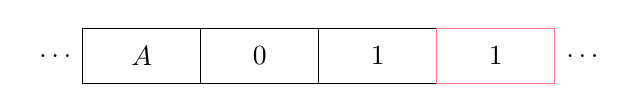
\begin{tikzpicture}
\begin{scope}[start chain=1 going right, node distance=-0.15mm]
    \node [on chain=1,tmtape,draw=none] {$\ldots$};
    \node [on chain=1,tmtape,large] {$A$};
    \node [on chain=1,tmtape,large] {0};
    \node [on chain=1,tmtape,large] {1};
    \node [on chain=1,tmtape,large,current] {$1$};
    \node [on chain=1,tmtape,draw=none] {$\ldots$};
\end{scope}
\end{tikzpicture}

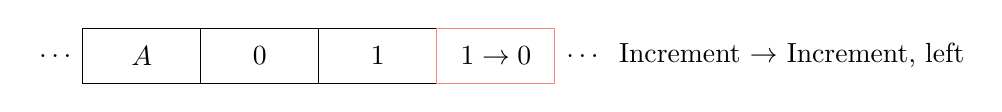
\begin{tikzpicture}
\begin{scope}[start chain=1 going right, node distance=-0.15mm]
    \node [on chain=1,tmtape,draw=none] {$\ldots$};
    \node [on chain=1,tmtape,large] {$A$};
    \node [on chain=1,tmtape,large] {0};
    \node [on chain=1,tmtape,large] {1};
    \node [on chain=1,tmtape,large,current] {$1 \to 0$};
    \node [on chain=1,tmtape,draw=none] {$\ldots$};
    \node [on chain=1] {Increment $\to$ Increment, left};
\end{scope}
\end{tikzpicture}

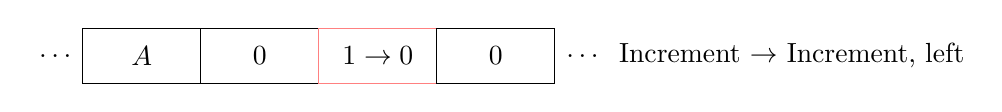
\begin{tikzpicture}
\begin{scope}[start chain=1 going right, node distance=-0.15mm]
    \node [on chain=1,tmtape,draw=none] {$\ldots$};
    \node [on chain=1,tmtape,large] {$A$};
    \node [on chain=1,tmtape,large] {0};
    \node [on chain=1,tmtape,large,current] {$1 \to 0$};
    \node [on chain=1,tmtape,large] {0};
    \node [on chain=1,tmtape,draw=none] {$\ldots$};
    \node [on chain=1] {Increment $\to$ Increment, left};
\end{scope}
\end{tikzpicture}

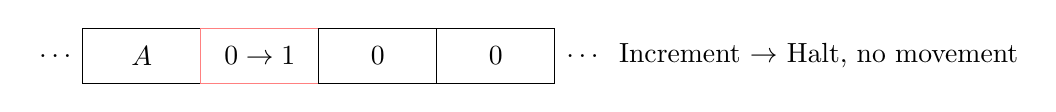
\begin{tikzpicture}
\begin{scope}[start chain=1 going right, node distance=-0.15mm]
    \node [on chain=1,tmtape,draw=none] {$\ldots$};
    \node [on chain=1,tmtape,large] {$A$};
    \node [on chain=1,tmtape,large,current] {$0 \to 1$};
    \node [on chain=1,tmtape,large] {0};
    \node [on chain=1,tmtape,large] {0};
    \node [on chain=1,tmtape,draw=none] {$\ldots$};
    \node [on chain=1] {Increment $\to$ Halt, no movement};
\end{scope}
\end{tikzpicture}

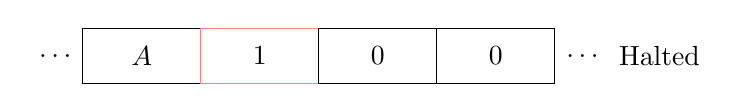
\begin{tikzpicture}
\begin{scope}[start chain=1 going right, node distance=-0.15mm]
    \node [on chain=1,tmtape,draw=none] {$\ldots$};
    \node [on chain=1,tmtape,large] {$A$};
    \node [on chain=1,tmtape,large,current] {1};
    \node [on chain=1,tmtape,large] {0};
    \node [on chain=1,tmtape,large] {0};
    \node [on chain=1,tmtape,draw=none] {$\ldots$};
    \node [on chain=1] {Halted};
\end{scope}
\end{tikzpicture}

The tape below is set up to increment 3 (011). It adds one getting 4 (100), carrying twice. Decrementing works the same way, except the $1$ and $0$ are switched, so 0 $\to$ 1, decrement $\to$ decrement (carry one), and 1 $\to$ 0,
decrement $\to$ halt.

\begin{tabular}{|l|l|l|l|l|l|}
\hline
Current state & Symbol read & Symbol wrote & Movement & Next state \\
\hline
Decrement & 1 & 0 & No movement & Halt \\
 & 0 & 1 & Left & Increment \\
 & $A$ & $A$ & No movement & Crash (underflow) \\
\hline
\end{tabular}

Not that when we try to decrement from the tape $A0000$, we find $0$ as the current symbol, change it to $1$, move to the left, and repeat (carry one). Then we find $0$ as the current symbol, change it to a $1$, move to the left, and repeat until we reach $A$ which tells us that the integer underflowed.


\subsection{Example Turing Program: Adding Natural Numbers}
Let our alphabet be the ${0, 1, A, B, C, D}$, where $0$ denotes a blank. We want to put the first number on the tape towards the left, and then the second number towards the right. In order for the Turing Machine to know where the numbers start and end, I will put an $A$ to denote the start of the first number, $B$ for its end, $C$ for the start of the second number, and $D$ for its end. Let the turing machine start anywhere to the right of $B$.

The following diagram is an example of the tap for this program set to compute 5 + 6. The 5 is between $A$ and $B$. The 6 is between $C$ and $D$. There can be an arbitrary amount of data between $B$ and $C$; It is all ignored by the program. This will become important later.

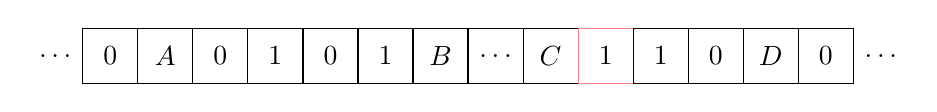
\begin{tikzpicture}
\begin{scope}[start chain=1 going right, node distance=-0.15mm]
    \node [on chain=1,tmtape,draw=none] {$\ldots$};
    \node [on chain=1,tmtape] {0};
    \node [on chain=1,tmtape] {$A$};
    \node [on chain=1,tmtape] {0};
    \node [on chain=1,tmtape] {1};
    \node [on chain=1,tmtape] {0};
    \node [on chain=1,tmtape] {1};
    \node [on chain=1,tmtape] {$B$};
    \node [on chain=1,tmtape] {$\ldots$};
    \node [on chain=1,tmtape] {$C$};
    \node [on chain=1,tmtape,current] {1};
    \node [on chain=1,tmtape] {1};
    \node [on chain=1,tmtape] {0};
    \node [on chain=1,tmtape] {$D$};
    \node [on chain=1,tmtape] {0};
    \node [on chain=1,tmtape,draw=none] {$\ldots$};
\end{scope}
\end{tikzpicture}

In general want to decrement the first number and increment the second number until the first number is zero. Then we know the sum is stored where the second number used to be second number (between $C$ and $D$).

\begin{enumerate}
\item In the style of the first example, I will navigate to the start of the first number (denoted by $B$) using the state `rewind'. This state moves to the left until it hits a $B$, and then moves exactly once more to the left.

\item Using the second example, I will decrement the first number by one under the state `decrement'. If the there is an underflow, that means I tried to decrement from zero, therefore the machine is done adding and it should halt.

\item Otherwise I want the machine to move back to the start of the second number (deonted by $D$) under state `forward'.

\item Now that the head is positioned, I want to increment the second number by one using the `increment' state. If there is an integer overflow, the second block of memory is not large enough to store the result, so the machine crashes. Otherwise repeat.
\end{enumerate}

\begin{tabular}{|l|l|l|l|l|l|}
\hline
Current state & Symbol read & Symbol wrote & Movement & Next state \\
\hline
Rewind & B & B & Left & Decrement \\
 & \textit{Otherwise} & \textit{None} & Left* & Rewind \\
\hline
Decrement & 1 & 0 & Right & Forward \\
 & 0 & 1 & Left & Decrement \\
 & A & A & None & Halt \\
\hline
Forward & D & D & Left & Increment \\
 & \textit{Otherwise} & \textit{None} & Right* & Forward \\
\hline
Increment & 0 & 1 & Left & Rewind \\
 & 1 & 0 & Left & Increment \\
 & C & C & None & Crash \\
\hline
\end{tabular}

Note that the program sets the first addend, $AB$, (where $xy$ means the number between $x$ and $y$) to zero while it sets the second addend $CD$ to the sum. If we want to reverse these roles, we simply change `left*' to `right' and `right*' to `left' (the asterisk is ignored by the Turing Machine; it used as a marker for educational purposes).

\subsection{Example Turing Program: Multiplying Natural Numbers}
Multiplication is repeated addition. The adder we built previously decrements its first input until it is zero, while the second input stores the result. In order to add numbers multiple times, we will need an adder that doesn't destroy first input. The second input will act as an accumulator for the sum, so it doesn't have to be reset.

In order to construct multiplication, we need another memory block delimited by $EF$ which starts out at zero. We will decrement the number in $AB$, then increment the number in $CD$ (like before), but then we will also increment the number in $EF$ before repeating. In the interest of time, the implementation will not be shown here. Instead, it is summarized below.

\begin{enumerate}
\item Decrement $AB$, go to step 5 on underflow.
\item Increment $CD$, crash on overflow.
\item Increment $EF$, crash on overflow
\item Repeat \\ (when loop terminates, $-1 \to AB$, $AB + CD \to CD$ $AB \to EF$)
\item Decrement $EF$, go to step 8 on underflow
\item Increment $AB$, crash on overflow
\item Repeat \\ (when loop terminates, $AB \to AB$, $AB + CD \to CD$, $-1 \to EF$)
\item Zero EF \\ (when program halts, $AB \to AB$, $AB + CD \to CD$, $0 \to EF$)
\end{enumerate}

Zero EF is a state that starts at F, if E is found halt, otherwise write zero, move to the left and repeat. Note that $-1$ denotes the number you get when you decrement one from zero (the number with a $1$ at every digit).

Notice that the `add, preserve first input' program can be used to copy one block of memory ($AB$) to another place ($CD$) provided that the other place is zero, using a temporary buffer ($EF$). This is because $AB \to AB$ so it remains unmodified. $AB + CD \to CD$, but $CD = 0$, so $AB \to CD$. Thus we can copy $AB$ to $CD$. By changing the direction of the adding we can even copy $CD$ to $AB$.

Now we have the tools to calculate $m \cdot n$. Let the $0 \to AB$, $m \to CD$ , $n \to EF$, and $0 \to GH$.

$AB$ is used as a counter to tell us how many times to add $CD$ to $EF$. When we add $CD$ to $EF$, we use `add, preserve first input' such that $CD$ is unchanged and $EF$ accumulates the result while $GH$ is used as a temporary buffer. The algorithm is summarized below.

\begin{enumerate}
\item Copy $CD$ to $AB$
\item Decrement $AB$ by one, halt on underflow.
\item Add, preserving the first input, $CD$ to $EF$ using $GH$ as a temporary buffer, storing the result in $CD$ (remember that this program needs a temporary storage buffer). Crash on overflow.
\item Repeat, starting from step 2. \\
(when the program halts, $-1 \to AB$, $CD \to CD$, $CD \cdot EF \to EF$, $0 \to GH$)
\end{enumerate}

\subsection{Example Turing Program: Computing Natural exponents}
We want to calculate $m^n$ for two natural numbers $m$ and $n$. Let the tape be set up where $n \to AB$, $0 \to CD$, $m \to EF$, $1 \to GH$, and $0 \to IJ$. We will decrement $AB$ until underflow, each time multiplying $EF$ and $GH$.

\begin{enumerate}
\item Decrement $AB$, halt on underflow
\item Multiply using $CD$ (storage), $EF$ ($m$), $GH$ ($n$), $IJ$ (storage), crash on overflow (Remember, $-1 \to CD$, $EF \to EF$, $EF \cdot GH \to GH$, $0 \to IJ$; Notice that $GH$ is used to store the second factor and the result is written to $GH$, so during the next iteration, the result of the previous iteration is multiplied by $EF$)
\item Repeat.
\end{enumerate}

\subsection{The Halting Problem}
Through out all of these programs there is recursion (meaning a repeating loop that calls itself). For example consider the, ``Search for character'' program
 
\begin{tabular}{|l|l|l|l|l|l|}
\hline
Current state & Symbol read & Symbol wrote & Movement & Next state \\
\hline
Rewind & B & B & No movement & Halt \\
 & 0 & 0 & Left & Rewind \\
 & 1 & 1 & Left & Rewind \\
\hline
\end{tabular}

What happens if the head starts out to the left of the $A$ instead of to the right? What happens if there is no $A$ on the tape? In these cases the Turing Machine goes into an infinite loop.

There is in fact no way to tell if any program will halt in finite time. Sometimes, like in the cases stated above with the ``Search for character'' program, we know that the program is going to be in an infinite loop if $A$ does not occur, but you could imagine a more difficult program that has thousands of states. While we do know that some programs won't halt given certain conditions, there are some programs for which we don't know if it will halt.

\section{Axiomatic systems}
\subsection{What is an axiomatic system?}
% The most common way of specifying an interpretation (especially in mathematics) is to specify a structure (also called a model; see below)

You should remember first-order logic has names (also called constants) denoted by lower case letters $a, b, c$. It also has predicates denoted as $Pxy$ or $P(x,y)$ (where the predicate $P$ is acting over the arguments $x$ and $y$) that evaluate too booleans. Thus $Px$ is usually true or false. There are also functions denoted the same way as predicates that evaluate to objects, so $f(x)$ is not true or false, but rather some object like $x$ or $2$ for example. There are also logical connectives like $\wedge$, and most importantly the quantifers $\exists$ and $\forall$.

An axiomatic system is a set of sentences in quantificational logic that describe something. These are very useful in mathematics. Natural numbers can be defined as an axiomatic system.

\subsection{Example Axiomatic System: Natural Numbers}
Let $Nx$ mean $x$ is a natural number, and $Sx$ mean the next number after $x$ (also called successor of $x$).
\begin{enumerate}
\item $\neg \exists x (Sx = 0)$ There is not a number whose successor is zero.
\item $\forall x \forall y (Sx = Sy \rightarrow x = y)$ Equal successors ($Sx = Sy$) mean equal numbers $x = y$.
\item $\forall y (\neg y = 0 \rightarrow (\exists x Sx = y))$ Except for zero, every number $y$ is the successor of some number $x$.
\item $\forall x (x + 0 = x)$ Identity property of addition.
\item $\forall x \forall y (x + S(y) = S(x + y))$ Defines addition recursively (together with the identity property)
\item $\forall x (x \cdot 0 = 0)$ Zero property of multiplication
\item $\forall x \forall y (x \cdot Sy = x \cdot y + x)$ Defines multiplication recursively (together with the identity property)
\item $(P(0) \wedge \forall k (P(k) \rightarrow P(k + 1))) \rightarrow \forall n P(n)$ A statement of induction
\end{enumerate}

This is called \textit{Peano Arithmetic}. There are many different versions, here is a common one. It encodes natural numbers in first-order logic.

\subsection{Models}
You should also remember that we can specify an \textit{interpretation} which is just an example of objects that satisfy make all of the sentences true. We specified models by creating a \textit{model}, which states the universe of discourse and specifying when predicates are true.

The Natural numbers you know are a model for Peano Arithmetic. $UD = \{0, 1, 2, \ldots\}$ where $S = \{(0, 1), (1, 2), \ldots\}$

% What does this even mean? I forgot how this is relevant
% There are also other models that satisfy the axioms called `non-standard models'. Let the $UD = \{0, 1, 2, \ldots, A, B, C, \ldots Z\}$ where $S(0) = \{(0, 1), (1, 2), \ldots\ (A, B), (B, C) \ldots (Z, A)}$ (the universe of discourse is natural numbers and letters, where the successor of a natural number is the next natural number and the successor of a letter is the next letter in the alphabet with the exception that $Z$ wraps around to $A$). This is also a model for Peano Arithmetic, but it is not the natural numbers. There is no contradiction here, even though the natural numbers don't work as expected.

\subsection{Completness and Consistency}
A formal system consists of syntax and semantics. Syntax tells us how to use the symbols to produce statements. Semantics tells us how to use the statements to deduce other statements. While syntax tells us how the language `sounds', semantics tells us what language `means'.

A formal system is complete if and only if every statement can be proven either true or false. A formal system is consistent if and only if no statement can be proven true and false.

% I don't even know if this is true
%There are not any good ways to `proove' consistency. We generally show consistency for a formal system, A, by showing that consistency of a simpler (more self-evident) system, consistency implies consistency of A. We

% This is how to prove inconsistency.

\subsection{Entscheidungsproblem}
David Hilbert proposed several famous questions. One of them asks for a procedure to determine if a sentence in first-order logic was valid (recall valid means true for every case that satisfies the premises). It is calling for a why to prove things that always works.

We studied Natural Deduction as a way to prove things in first-order logic. This sometimes works. Consider a invalid argument. Natural deduction will deduce things that are true, but when using natural deduction there are some arguments that can't be shown to be valid or invalid.

Consider the following argument which can neither be proven true nor proven false using natural deduction.

\begin{tabular}{l}
$\exists x Px$ \\
$\exists y Py$ \\
\hline
$\exists x (Px \wedge Py) $ \\
\end{tabular}

With these premises, we can never deduce $\exists x (Px \wedge Py) $ or $\neg \exists x (Px \wedge Py) $. Natural deduction continues indefinately, not proving this statement.

\section{Observations}
\subsection{Church-Turing Hypothesis}
The Church-Turing thesis proved that three methods of formalizing the idea of computability were all equivalent, and that these methods coincide with the informal notion of an effectively calculatable function. Informally, an \emph{effectively calulatable function} can be done by a human with a pencil and paper, ignoring resource limitations (including time). The three methods of formalizing computability were:

\begin{enumerate}
\item Kurt G\"{o}del and Jacques Herbrand's idea of the General Recursive Function.
\item Alonzo Church's method called the $\lambda$-calculus
\item The Turing machine
\end{enumerate}

This is important because it says that if I want to see if my computer is capable of computing any function (barring memory and time constraints), I can see if it can simulate a Turing Machine, or see if I can implement Lambda Calculus, or see if I can encode recursive functions. If any of these are possible, my computer is powerful enough to theoretically calculate anything (within time and memory constraints).

This is most significant because if a problem is unsolvable with a Turing machine, then the problem must be incomputable. No other method could possibly solve it. But what problems could possibly fall into this category?

\subsection{G\"odel's Incompleteness Theorems}
\textbf{G\"odel's First Incompletness Theorem} Every set of axioms is either inconsistent or incomplete, where incomplete means that it cannot prove all truths about the natural numbers.\\\textbf{G\"odel's Second Incompletness Theorem} The second incompleteness theorem shows that such a system cannot demonstrate its own consistency.

\subsection{Informal proof}
Lets say we have a set of axioms, $S$. Assume $S$ is complete. Since $S$ is complete, we can write a computer program, $P$, and prove ``$P$ halts'' or ``$P$ doesn't halt'' using rules from $S$.

Let $P$ be a program that makes a copy of itself, called $R$, and uses rules of $S$ to prove ``$R$ does not halt.'' Once it proves this, $P$ halts.

Notice if $P$ halts, it must have proven ``$R$ does not halt,'' but $R$ is a copy of $P$, therefore $P$ does not halt. Contradiction

If $P$ does not halt, then ``$R$ does not halt'' must be not provable in finite time. Thus there are statements in $S$ that can't be proven. Therefore $S$ is inconsistent. Contradiction.

Thus G\"odel's first Incompletness Theorem is proven. %The second can be proven by changing the example a bit.

%Let $P$ be a program that makes a copy of itself, called $R$, and uses rules of $S$ to prove either ``$R$ produces output'' or ``$R$ does not produce output''. If $R$ produces output, halt. If $R$ produces no output, output ``Hello world'' and halt.

%If $P$ produces output, $R$ did not produce output, but $R$ is a copy of $P$, therefore $S$ proved $P$ does not produce output even though $P$ produces output. If $P$ halts without output, $R$ did produce output, but $R$ is a copy of $P$, therefore $S$ proved $P$ does produce output even though it doesn't.

%At this point, $P$ halts or it doesn't. If it halts, $S$ is contradictory (it proved $P$ produces output and $P$ doesn't produce output). If it does not halt $S$ is incomplete (it can't prove $P$ produces output or $P$ doesn't produce output). 

% Wait how does this prove Godel's second?
\subsection{Incompleteness implications: Entscheidungsproblem}
Any proof system in first-order logic is either incomplete or inconsistent, which means that we cannot fully analyze a program, which informally means that we cannot deduce if a statement is universally valid. G\"odel's work influenced the work of Turing and Church heavily, but it was not sufficient to rigorously solve the Entscheidungsproblem.

\subsection{Incompleteness implications: Halting problem}
We can't be sure that a given turing program will halt. We know this because the program cannot be fully analyzed, as informally implied by G\"odel, so we will not be able to fully deduce the fate of the program. Again, the work of G\"odel laid the foundation for future research, but it was insufficient to formally solve the halting problem.

\subsection{Incompletness implications: Continued implications}
You can't prove \textit{everything} in first-order logic. There will always things which you can not prove. 

The laws of physics in our universe can emulate a Turing machine (since we have built real life Turing machines), therefore the laws of physics in our universe is at least as powerful as a Turing machine.

Some claim it is equal in power to a Turing machine (there exists a precise set of rules, even probabilistic rules, to model nature). This implies that every physical situation in the universe is computable. All the laws of physics can be simulated by a computer and described through numbers. This is called digital physics, and it contradicts some of quantum physics, so most people are skeptical.

The other option is that it is greater in power than a Turing machine, in which case could we use physical phenomena to create a computer more powerful than a Turing machine? This idea has been termed the hypercomputer. Still others speculate that althought the universe contains physical phenomena that can not be simulated with a Turing machine, this phenomena is not `harnessable' for the construction of a hypercomputer. 


\end{document}

%%% Local Variables: 
%%% mode: latex 
%%% TeX-master: t 
%%% End:
